\documentclass[a4paper,12pt,pointlessnumbers]{scrartcl}
\usepackage[utf8]{inputenc}
\usepackage[ngerman]{babel}
\usepackage{fontenc}
\usepackage{hyperref}
\usepackage{url}
\usepackage{listings}
\usepackage{color}
\usepackage{framed}
\usepackage{acronym}
\usepackage{graphicx}
\usepackage{marginnote}

\setlength{\parindent}{0pt}
% \setlength{\parskip}{0ex}

% Title Page
\title{CMS Pixeldetektorupgrade Phase 1\\---\\Handbuch\\---\\HDI Test}
\author{Benedikt Vormwald -- Universit\"{a}t Hamburg}


\definecolor{myblue}{rgb}{0.86,0.90,1.00}
\definecolor{mygreen}{rgb}{0.76,0.9,0.7}

\lstdefinestyle{console1}{
  basicstyle=\ttfamily,
  backgroundcolor=\color{myblue},
  frame=single,
  framerule=0pt
}

\lstdefinestyle{console2}{
  basicstyle=\ttfamily,
  backgroundcolor=\color{mygreen},
  frame=single,
  framerule=0pt
}


\newcommand{\warnung}[1]{\marginnote{
\includegraphics[width=8mm]{./figures/warnung.png}}\textbf{#1}}
\newcommand{\protokoll}[1]{\marginnote{
\includegraphics[width=5mm]{./figures/protokoll.png}}\textbf{#1}}




\begin{document}
\maketitle
\begin{abstract}
Dieses Handbuch beschreibt schrittweise die Durchf\"{u}hrung des Tests des HDI im Zusammenhang mit der Pixeldetektor-Modulproduktion 2015 an der Universit\"{a}t Hamburg f\"{u}r das Phase1-Upgrade des CMS Pixeldetektors.
\end{abstract}

\tableofcontents
\newpage

\section{Kontaktpersonen}
Bei Problemen mit dem Messaufbau sowie bei unerwartetem Ergebnissen kontaktieren Sie
\textbf{Adrian Perieanu} (Telefon: 2115, B{\"u}ro: Geb. 68/ Raum 112) oder \textbf{Benedikt Vormwald} (Telefon: 2192, B{\"u}ro: Geb. 68/ Raum 123).

\section{Aufbau des Teststandes}
\begin{figure}
\centering
  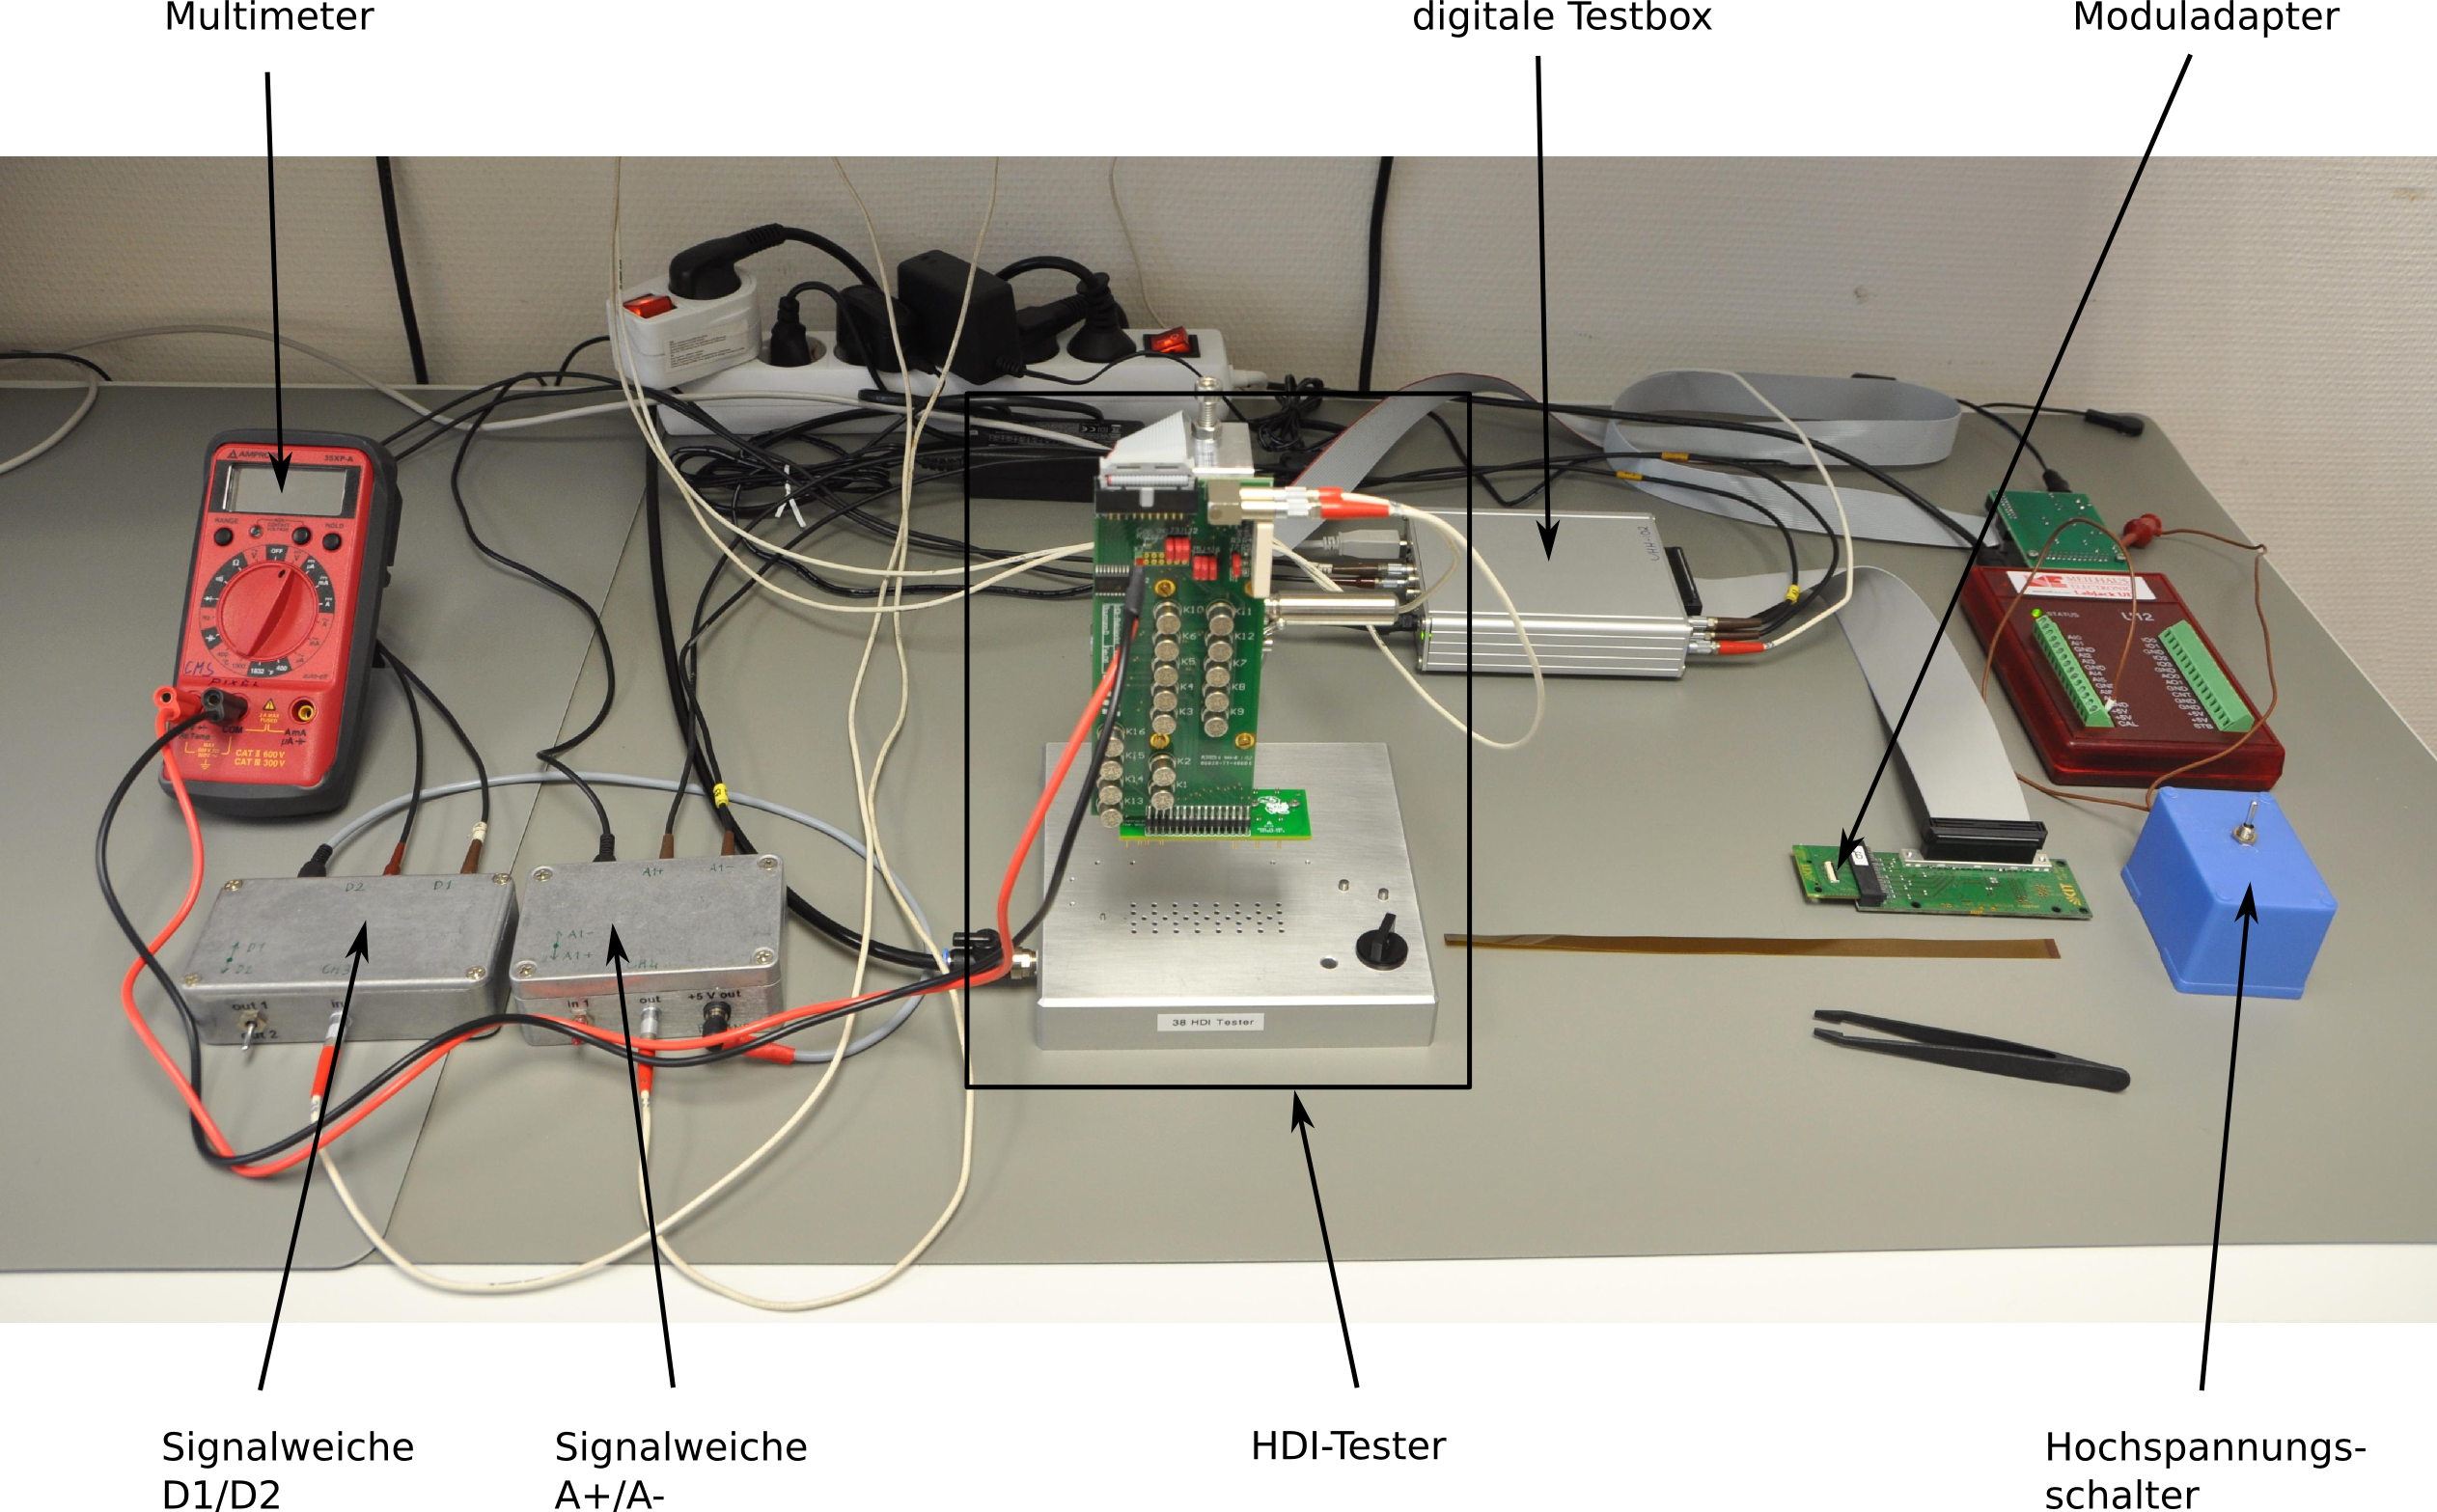
\includegraphics[angle=90]{figures/setup_labled.png}
 \caption{Setup.}
 \label{fig:setup}
\end{figure}
Abbildung~\ref{fig:cableconnection} zeigt den Aufbau des HDI-Teststandes.
Er besteht aus einem DAQ-Computer (nicht abgebildet), einer digitalen Testbox mit Moduladapter, zwei Signalweichen sowie ein Hochspannungsnetzteil (nicht abgebildet, Abbildung~\ref{fig:sourcemeter}) mit Hochspannungsschalter und einem Oszilloskop (nicht abgebildet, Abbildung~\ref{fig:scope}).
Das Kernst{\"u}ck des Messaufbaus bildet der HDI-Tester (Abbildung~\ref{fig:hditester}).
Der Messkopf des HDI-Testers kann auf eine Arbeitsplattform abgesenkt werden um dort ein HDI zu kontaktieren.
Den elektrischen Kontakt stellt die Nadelkarte her, w{\"a}hrend die Relaiskarte die angesteuerten Nadeln regelt.
\begin{figure}
\centering
  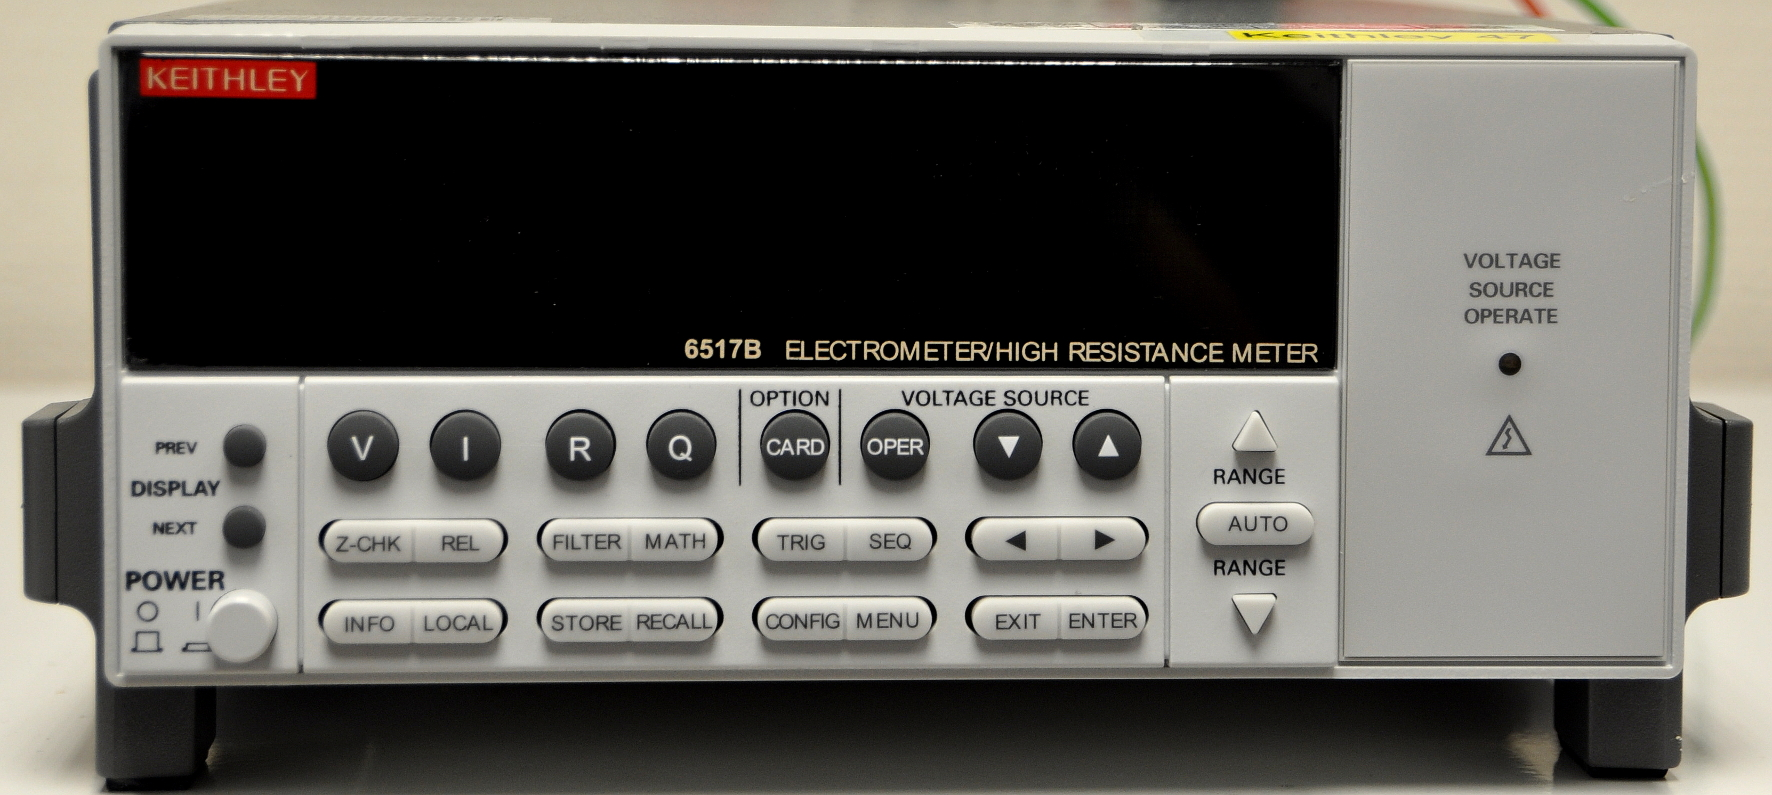
\includegraphics[width=0.8\textwidth]{figures/sourcemeter.jpg}
 \caption{Hochspannungsquelle \texttt{Keithley 6517B}.}
 \label{fig:sourcemeter}
\end{figure}
\begin{figure}
\centering
  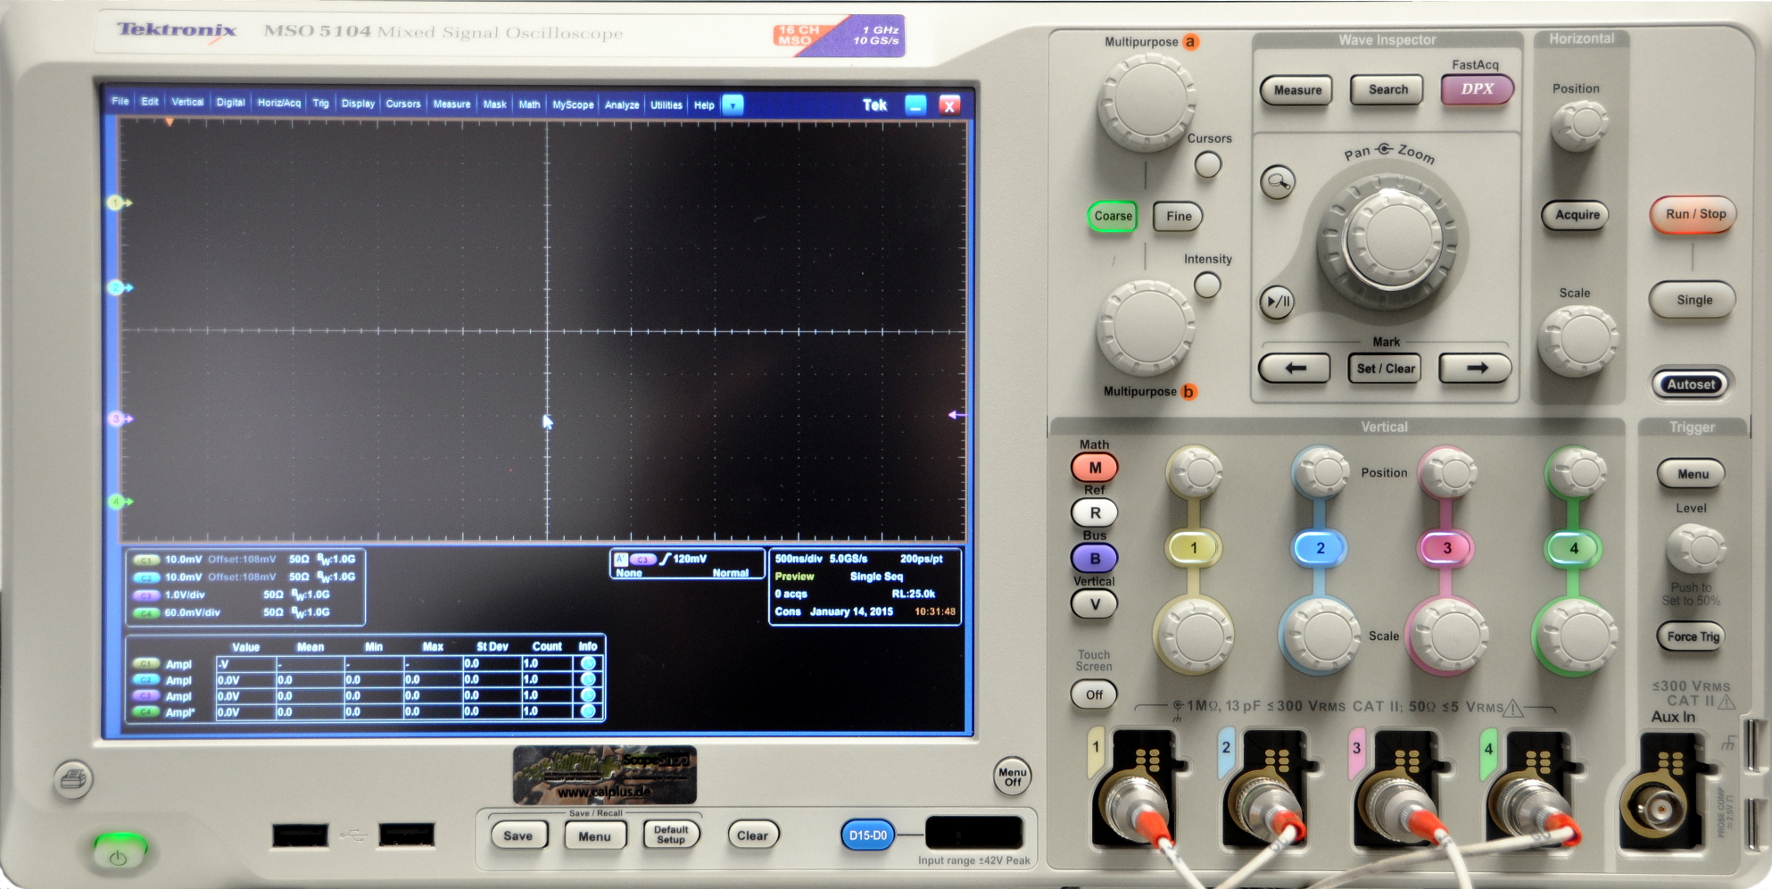
\includegraphics[width=\textwidth]{figures/scope.jpg}
 \caption{Oszilloskop \texttt{Tektronix MSO 5104}.}
 \label{fig:scope}
\end{figure}
\begin{figure}
\centering
  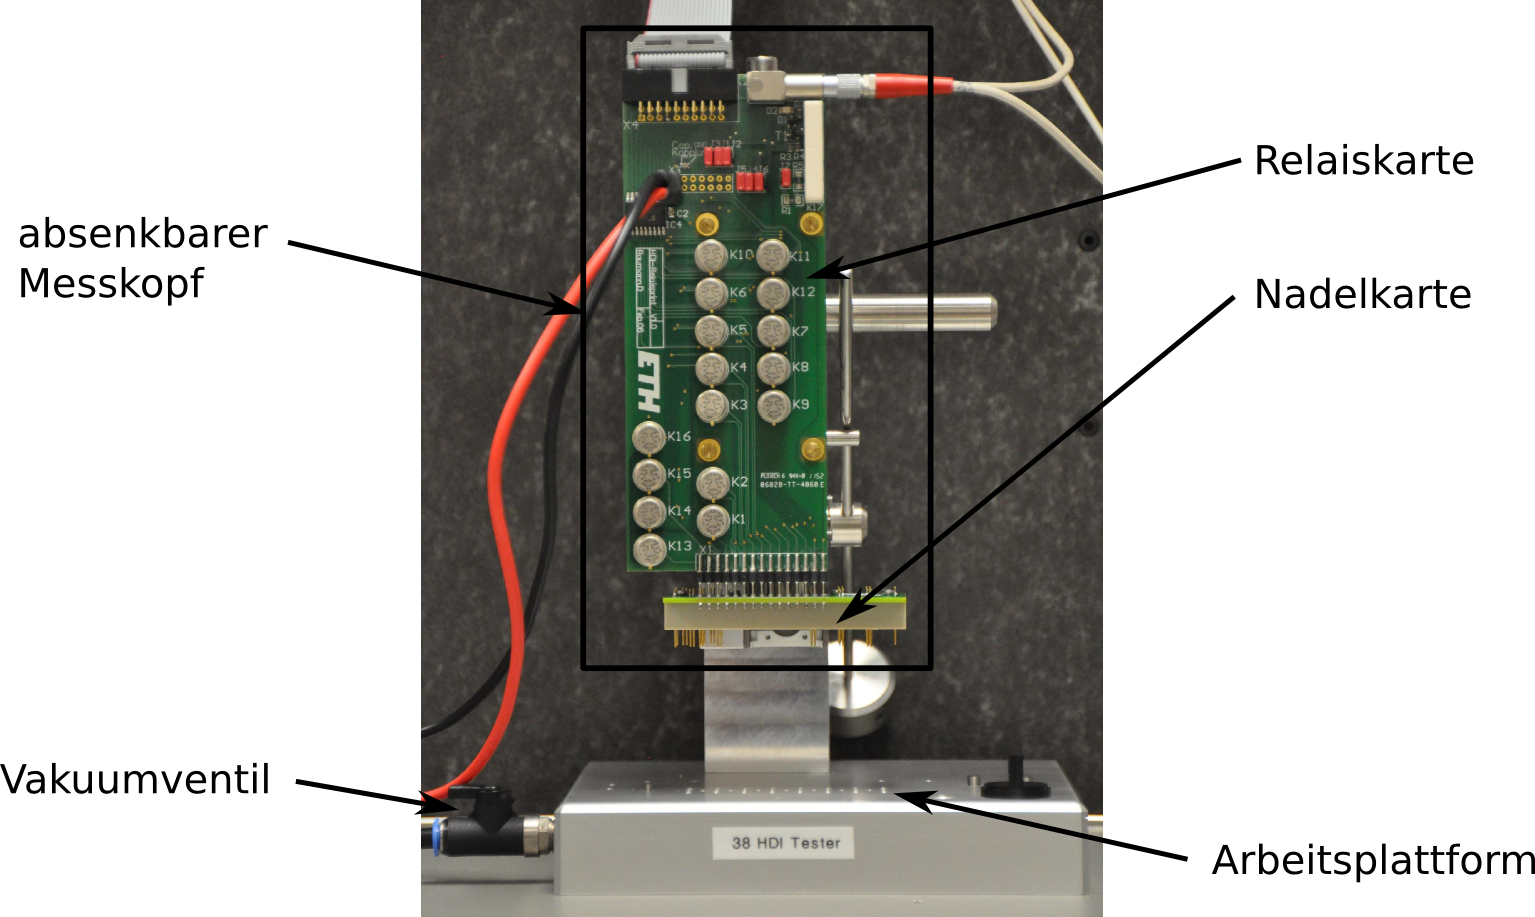
\includegraphics{figures/hditester_labled.png}
 \caption{HDI-Tester.}
 \label{fig:hditester}
\end{figure}



\section{Sichtkontrolle}
Bevor Sie die Tr{\"a}gerplatte mit dem HDI in den HDI-Tester installieren und mit den elektronischen Tests beginnen erfolgt eine Sichtkontrolle des HDIs.
Beachten Sie dabei, dass das HDI \warnung{unter keinen Umst{\"a}nden direkt mit den Fingern ber{\"u}hrt} werden darf, da die Ablagerung von Hautfett die sp{\"a}teren Prozessschritte behindert.
Fassen Sie daher stets ausschlie{\ss}lich die Tr{\"a}gerplatte an.

\"Uperpr\"ufen Sie mit Hilfe des Mikroskops oder einer Lupe, ob die wire-bonds korrekt das HDI mit dem TBM-Chip verbinden.
Die Verbindungen sollten vollst{\"a}ndig sein, parallel zueinander ausgerichtet sein und sich gegenseitig nicht ber{\"u}hren.
\"Uberpr\"ufen Sie das HDI auch auf sonstige mechanische Deformationen und vermerken Sie \protokoll{Auff\"alligkeiten} im Testprotokoll.
%Die Sichtkontrolle wird am Ende der elektronischen Tests nochmals wiederholt.
Notieren Sie in diesem Schritt auch die \textbf{Identifikationsnummer des HDI} (vgl. Abbildung \ref{fig:hdi}).

\begin{figure}
\centering
  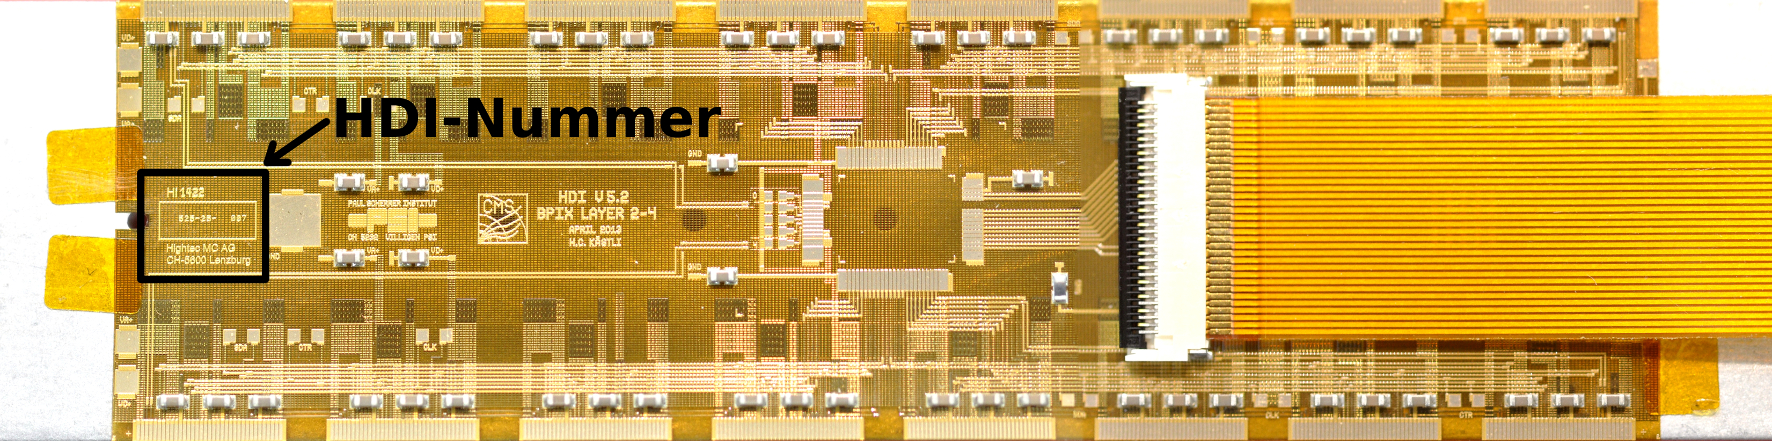
\includegraphics[height=0.15\textwidth]{figures/hdi_labled.jpg}
  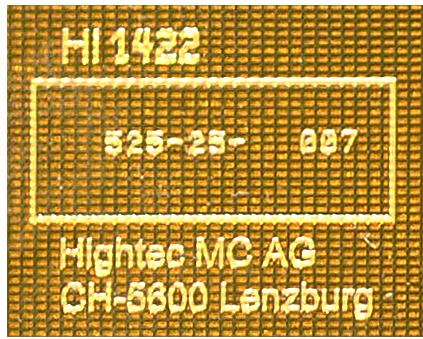
\includegraphics[height=0.15\textwidth]{figures/hdinummer.jpg}
 \caption{Visuelle {\"U}berpr{\"u}fung des HDIs. Die HDI-Nummer ist auf dem HDI eingepr{\"a}gt.}
 \label{fig:hdi}
\end{figure}

\section{Vorbereitung der elektronischen Tests}
Bet{\"a}tigen Sie den Kippschalter an der Steckdosenleiste um alle Ger{\"a}te mit Spannung zu versorgen.
Der zus{\"a}tzliche Kippschalter f{\"u}r die Vakuumpumpe sollte im Moment noch ausgeschaltet bleiben.
Schalten Sie daraufhin das Oszilloskop sowie das Keithley-Hochspannungsnetzteil ein.

In Vorbereitung auf den Hochspannungstest wird der Ausgangskanal des Netzteils f{\"u}r eine Spannung von 600V konfiguriert.
Beachten Sie dabei, dass der \warnung{Ausgangskanal in diesem Schritt noch nicht aktiviert wird}.
F{\"u}r die Konfiguration gehen Sie wie folgt vor:
\begin{itemize}
\item W{\"a}hlen Sie am Ger{\"a}t das Konfigurationsmen{\"u} f{\"u}r die Ausgabespannung aus (config-Taste sowie anschlie{\ss}end eine beliebige Taste im Bereich \frqq Voltage Source\flqq), selektieren Sie dort den Men{\"u}punkt \texttt{RANGE} und best{\"a}tigen Sie mit der enter-Taste.
\item W{\"a}hlen Sie den Spannungsbereich bis 1000V mit den Curser-Tasten (Pfeiltasten links-rechts), best{\"a}tigen Sie die Auswahl mit der enter-Taste und verlassen Sie das Men{\"u} wieder mit der exit-Taste.
\item Zur{\"u}ck auf der Hauptanzeige stellen Sie nun die Ausgabespannung mit den Curser-Tasten und Pfeil-Tasten im Bereich \frqq Voltage Source\flqq\ auf 600V ein.
Best{\"a}tigen sie in diesem Fall ihre Eingabe \textbf{nicht} mit der enter-Taste.
Das Ger{\"a}t wechselt nach einigen Sekunde von alleine aus dem Editiermodus in den Anzeigemodus.
\item  W{\"a}hlen Sie nun den Strommessmodus (Taste I), sodass die im Display angezeigte Gr{\"o}{\ss}e einen Strom darstellt.
\item  Mit den range-Tasten w{\"a}hlen Sie den Messbereich $20\mu\mathrm{A}$ aus.
\item  Deaktivieren Sie im letzten Schritt den Zero-Check (Z-CHK).
\end{itemize}



Installieren Sie nun die Tr{\"a}gerplatte mit dem HDI in den HDI-Tester.
Abbildung~\ref{fig:mounting} zeigt die einzelnen Schritte:
\begin{figure}[h]
\centering
  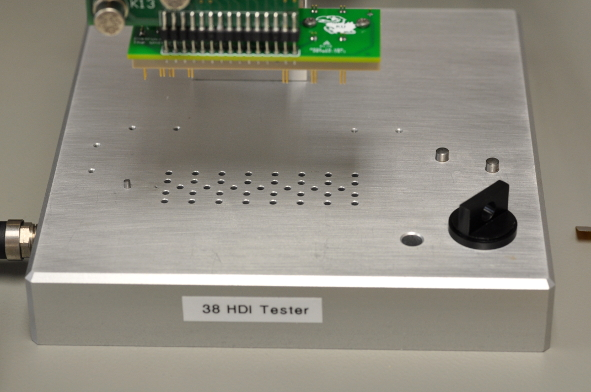
\includegraphics[width=0.3\textwidth]{figures/mounting1.jpg}
  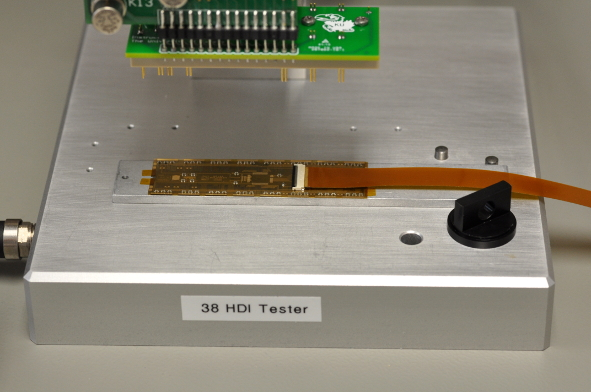
\includegraphics[width=0.3\textwidth]{figures/mounting2.jpg}
  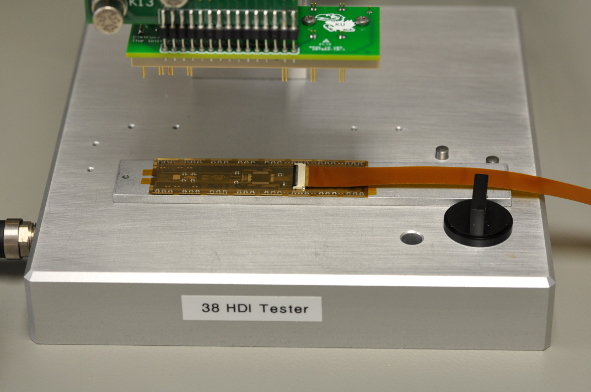
\includegraphics[width=0.3\textwidth]{figures/mounting3.jpg}
 \caption{Einsetzen der HDI-Tr{\"a}gerplatte in den HDI-Tester.}
 \label{fig:mounting}
\end{figure}
\begin{itemize}
\item Richten Sie die Tr{\"a}gerplatte so aus, dass die Bohrung auf den linken Stift des HDI-Testers passt.
Die Tr{\"a}gerplatte sollte flach auf der Arbeitsplattform des HDI-Tester aufliegen.
\item Drehen Sie anschlie{\ss}end an dem schwarzen Plastikknopf um die Tr{\"a}gerplatte gegen den hinteren Stift des HDI-Testers zu pressen.
\item Die so arretierte Tr{\"a}gerplatte wird nun durch Aktivieren der Vakuumpumpe zus{\"a}tzlich fixiert.
\end{itemize}

Verbinden Sie im n{\"a}chsten Schritt das Flachkabel, das bereits mit dem HDI verbunden ist, mit dem Moduladapter.
Abbildung~\ref{fig:cableconnection} zeigt das Vorgehen:
\begin{figure}[h]
\centering
  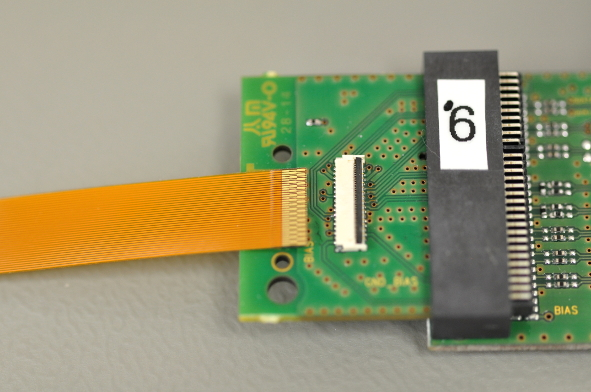
\includegraphics[width=0.3\textwidth]{figures/cableconnection1.jpg}
  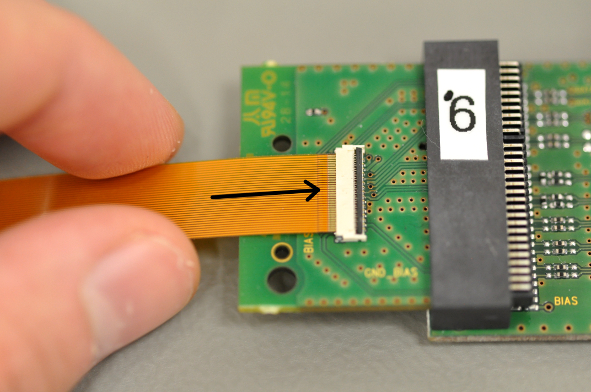
\includegraphics[width=0.3\textwidth]{figures/cableconnection2_labled.jpg}
  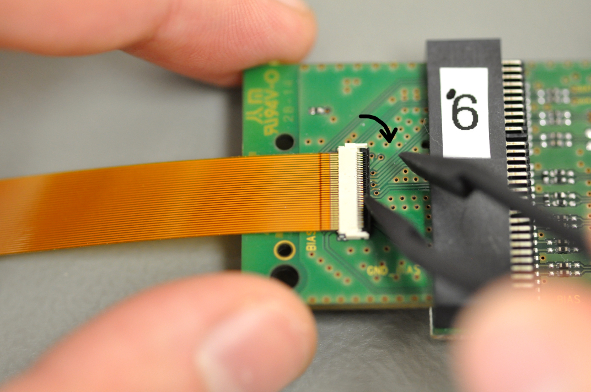
\includegraphics[width=0.3\textwidth]{figures/cableconnection3_labled.jpg}
 \caption{Schritte zum Verbinden des HDI-Flachkabels mit dem Moduladapter.}
 \label{fig:cableconnection}
\end{figure}
\begin{itemize}
\item Achten Sie darauf, dass die Kabelaufnahme am Moduldadapter ge{\"o}ffnet ist. Der schwarze B{\"u}gel muss dabei nach oben zeigen.
\item F{\"u}hren Sie nun das Flachkabel in die Kabelaufnahme ein bis sie einen Widerstand sp{\"u}hren.
\item Anschlie{\ss}end benutzen Sie eine Pinzette um den schwarzen B{\"u}gel auf die Seite zu klappen und damit das Kabel zu fixieren.
\end{itemize}
Die Fixierung des Flachkabels in der Kabelaufnahme erfordert einen etwas gr{\"o}{\ss}eren Kraftaufwand, weshalb unbedingt darauf zu achten ist, dass der \warnung{Moduladapter durch ein Abrutschen nicht besch{\"a}digt wird}.

Im n{\"a}chsten Schritt wird das HDI mit dem Nadelboard des HDI-Testers vorsichtig kontaktiert.
Abbildung~\ref{fig:slidingcarriage} zeigt die n{\"o}tigen Schritte:
\begin{figure}[h]
\centering
  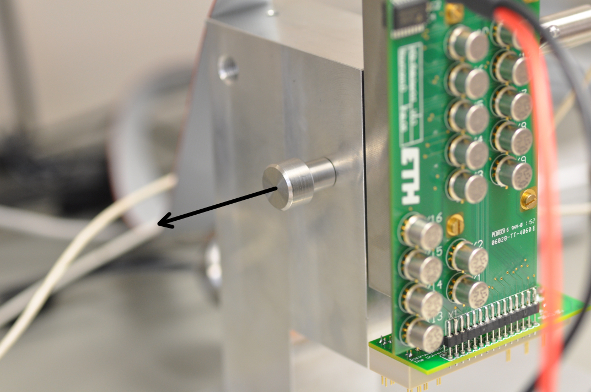
\includegraphics[width=0.3\textwidth]{figures/slidingcarriage2_labled.jpg}
  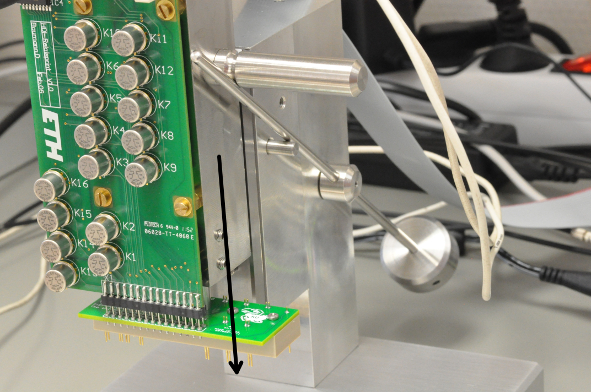
\includegraphics[width=0.3\textwidth]{figures/slidingcarriage1_labled.jpg}
  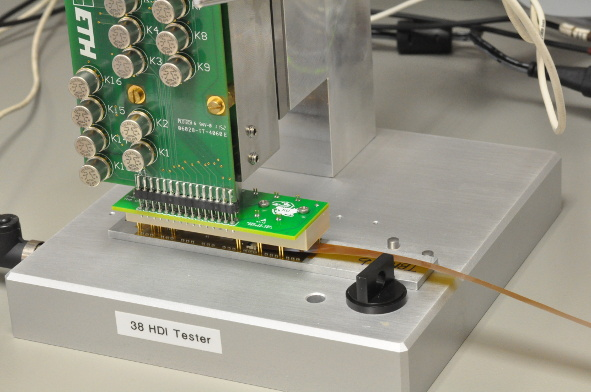
\includegraphics[width=0.3\textwidth]{figures/slidingcarriage3.jpg}
 \caption{Absenken des Nadelboards auf das installierte HDI.}
 \label{fig:slidingcarriage}
\end{figure}
\begin{itemize}
\item Um den Messkopf mit den Kontaktnadeln abzusenken ist es n{\"o}tig die Arretierung auf der linken Seite des HDI-Testers zu l{\"o}sen.
Der Sicherungsstift wird dazu etwa 2cm herausgezogen.
Beachten Sie, dass der Messkopf sehr schwer ist und \warnung{beim L{\"o}sen der Arretierung auf jeden Fall festgehalten werden muss}.
Unter keinen Umst{\"a}nden darf der Messkopf auf das HDI fallen, da dadurch sowohl das HDI als auch die empfindlichen Messspitzen zerst{\"o}rt werden.
\item Setzen Sie den Messkopf sehr behutsam auf das HDI.
\end{itemize}

Zuletzt bereiten Sie den DAQ-Computer vor.
F\"ur die folgenden elektronischen Tests werden zwei ge\"offnete Konsolenfenster (\colorbox{myblue}{\texttt{console 1}} \colorbox{mygreen}{\texttt{console 2}}) ben\"otigt.
Der Farbcode dient im Weiteren zur Unterscheidung zwischen den beiden Konsolenfenster.
Stellen Sie sicher, dass Sie in beiden Konsolen die richtigen Ordner ge{\"o}ffnet haben:
\begin{lstlisting}[style=console1]
 cd ~/psi46test
\end{lstlisting}
\begin{lstlisting}[style=console2]
 cd ~/HDItest/Lab-Jack-Code/examples
\end{lstlisting}

\section{Elektronische Tests}
\subsection{Test der Datensignalausgabe}
Im ersten Test wird die generelle Datensignalausgabe getestet.
Starten Sie daf{\"u}r das Kontrollprogramm f{\"u}r das Testboard:
\begin{lstlisting}[style=console1]
 bin/psi64test data/logfile.log
 > fsel 2
 > startmod
\end{lstlisting}
Wiederholen Sie den letzten Befehl bis f{\"u}r den digitale Strom in der Konsolenausgaben $\mathrm{I_D}\approx12\mathrm{mA}$ angezeigt wird.
$\mathrm{I_A}$ sollte stets $0\mathrm{mA}$ anzeigen.
Vermerken Sie den gemessenen \protokoll{Wert f{\"u}r $\mathrm{I_D}$} im Testprotokoll.

W{\"a}hlen Sie an der ersten Signalweiche \frqq D1\flqq\ als Synchronisationssignal und an der anderen Signalweiche \frqq A+\flqq.
Sie sollten nun ein auf dem Oszilloskopbildschirm ein Bild wie in Abbildung~\ref{fig:signaldifftest} sehen.

\begin{figure}
\centering
%   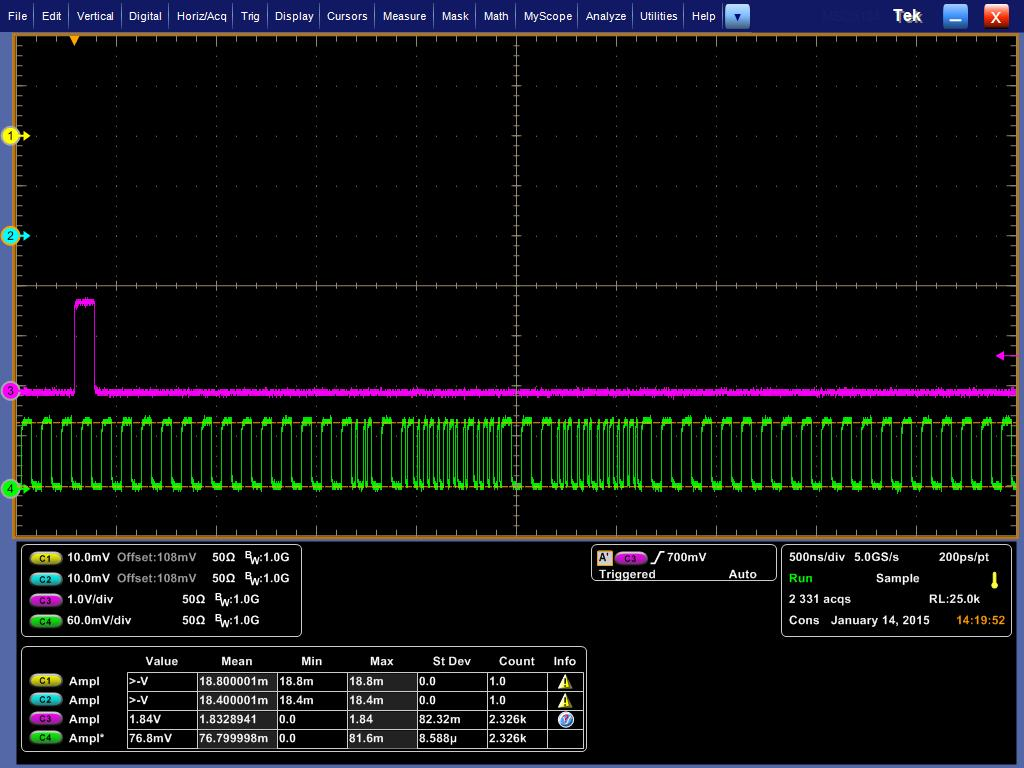
\includegraphics[width=0.45\textwidth]{figures/1_diffresp_minus.jpg}
  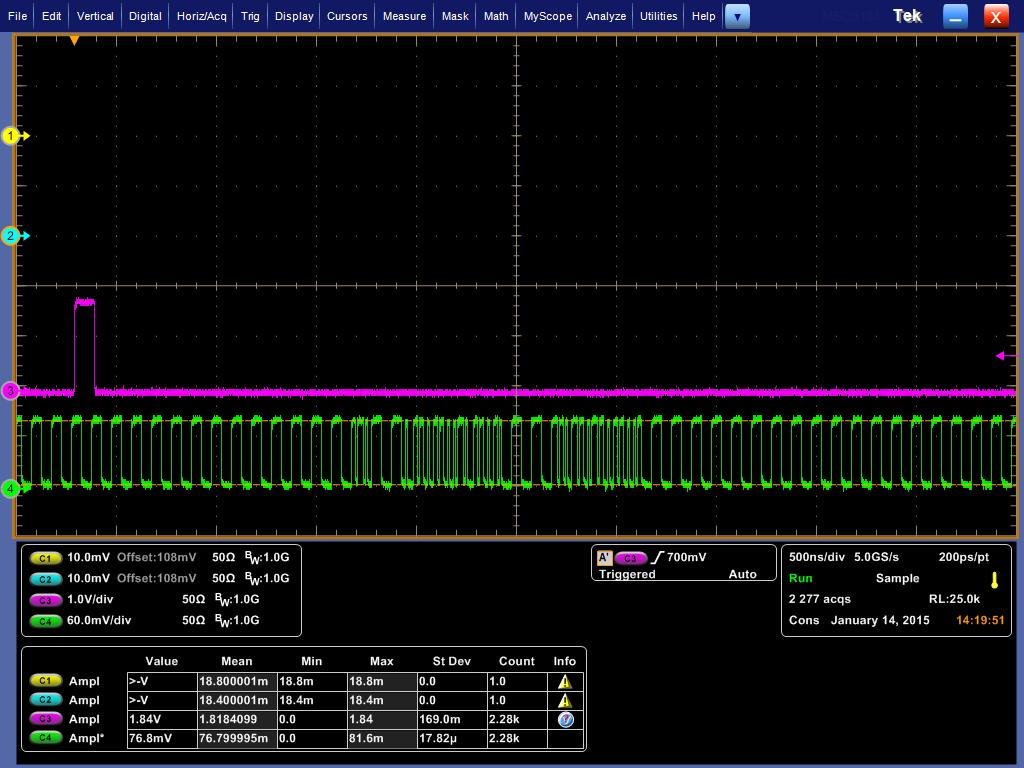
\includegraphics[width=0.7\textwidth]{figures/1_diffresp_plus.jpg}
 \caption{Oszilloskopbild beim TBM-Response-Test.}
 \label{fig:signaldifftest}
\end{figure}

{\"U}berpr{\"u}fen Sie, ob im Oszilloskopkanal 4 ein Rechtecksignal vorhanden ist, das in der Mitte des Bildausschnitts vom TBM-Header {\"u}berlagert ist.
Wiederholen Sie die {\"U}berpr{\"u}fung f{\"u}r die Auswahl \frqq A-\flqq\ an der zweiten Signalweiche.
Dies sollte ein invertiertes Bild vom Oszilloskopkanal 4 zeigen.
Vermerken Sie die \protokoll{Ergebnisse f{\"u}r \frqq A+\flqq\ und \frqq A-\flqq} im Testprotokoll.

\subsection{Clock-Test}\label{sec:clocktest}
Im n{\"a}chsten Schritt werden vier Clock-Signale getestet.
Schalten Sie dazu zun{\"a}chst die Relaiskarte an:
\begin{lstlisting}[style=console2]
 ./Poweron
\end{lstlisting}
F{\"u}hren Sie anschlie{\ss}end das folgende Programm aus:
\begin{lstlisting}[style=console2]
 ./Clock[0,1,2,3]
\end{lstlisting}
Das Oszilloskopbild sollte nun ein {\"a}hnliches Bild wie in Abbildung~\ref{fig:clocktest} zeigen.
\begin{figure}
\centering
  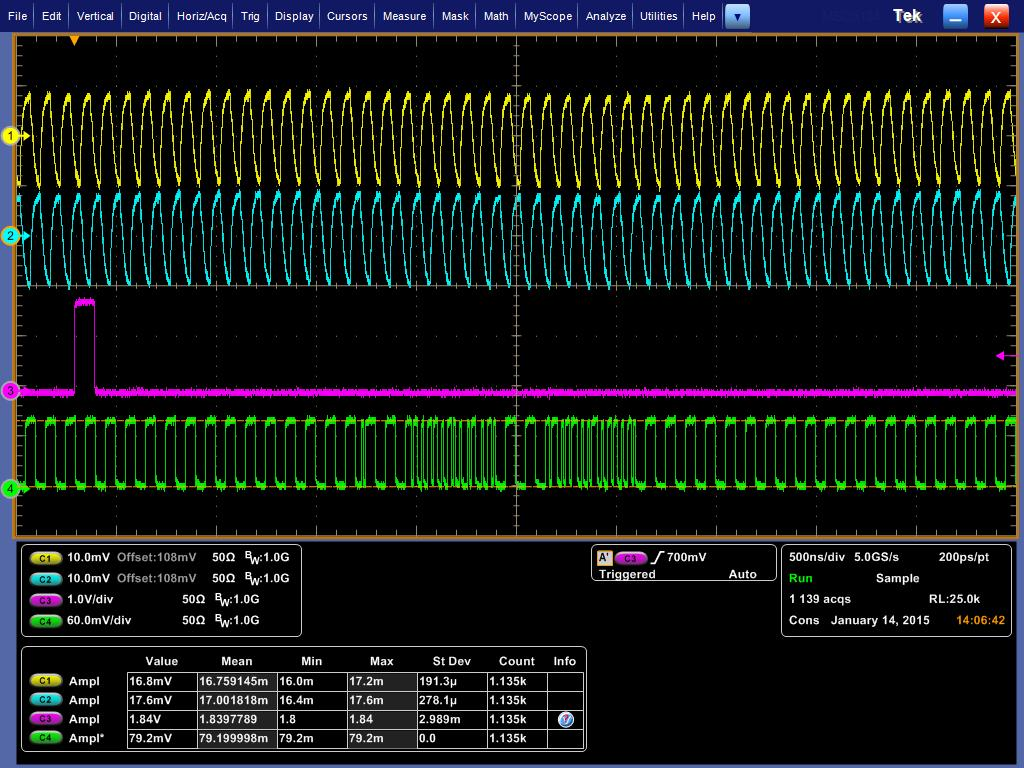
\includegraphics[width=0.7\textwidth]{figures/2_clock.jpg}
 \caption{Oszilloskopbild beim Clock-Test.}
 \label{fig:clocktest}
\end{figure}

Sollten die Amplituden im Oszilloskopkanal 1 und/oder 2 deutlich unter $20\mathrm{mV}$ betragen, ist das HDI wahrscheinlich nicht gut von den Messnadeln kontaktiert.
In diesem Fall kann oftmals die Kontaktierung verbessern werden indem die fixierte Tr{\"a}gerplatte etwas hin und her gedr{\"u}ckt wird.
Liefert dies nicht die gew{\"u}nschte Verbesserung heben Sie den Messkopf erneut ab und setzen ihn vorsichtig wieder auf das HDI auf.

Zur Ermittlung der Amplitude des Signals in Oszilloskopkanal 1 und 2 unterbrechen Sie am Oszilloskop den Run mit der Taste Run/Stop, w{\"a}hlen Sie dann die Taste Single und starten Sie anschlie{\ss}end erneut den Run.
Dieses Vorgehen ist wichtig um den Oszilloskopspeicher zu leeren, der benutzt wird um die mittlere Amplitude der Signale in den verschiedenen Oszilloskopkan{\"a}len zu bestimmen.

Lesen Sie nun die mittlere \protokoll{Amplitude f{\"u}r Oszilloskopkanal 1 und 2} im unteren Teil des Oszilloskopbildschirms ab und vermerken Sie die Werte im Testprotokoll.
Lesen Sie bei diesem Test au{\ss}erdem die \protokoll{Spannung am Multimeter} ab und vermerken Sie auch diesen Wert im Testprotokoll.


\subsection{CTR-Test}
F{\"u}r den Test der vier CTR-Signale f{\"u}hren Sie das folgende Programm aus:
\begin{lstlisting}[style=console2]
 ./CTR[0,1,2,3]
\end{lstlisting}

Das Signal auf dem Oszilloskopbildschirm sollte wie in Abbildung~\ref{fig:ctrtest} aussehen:
\begin{figure}
\centering
  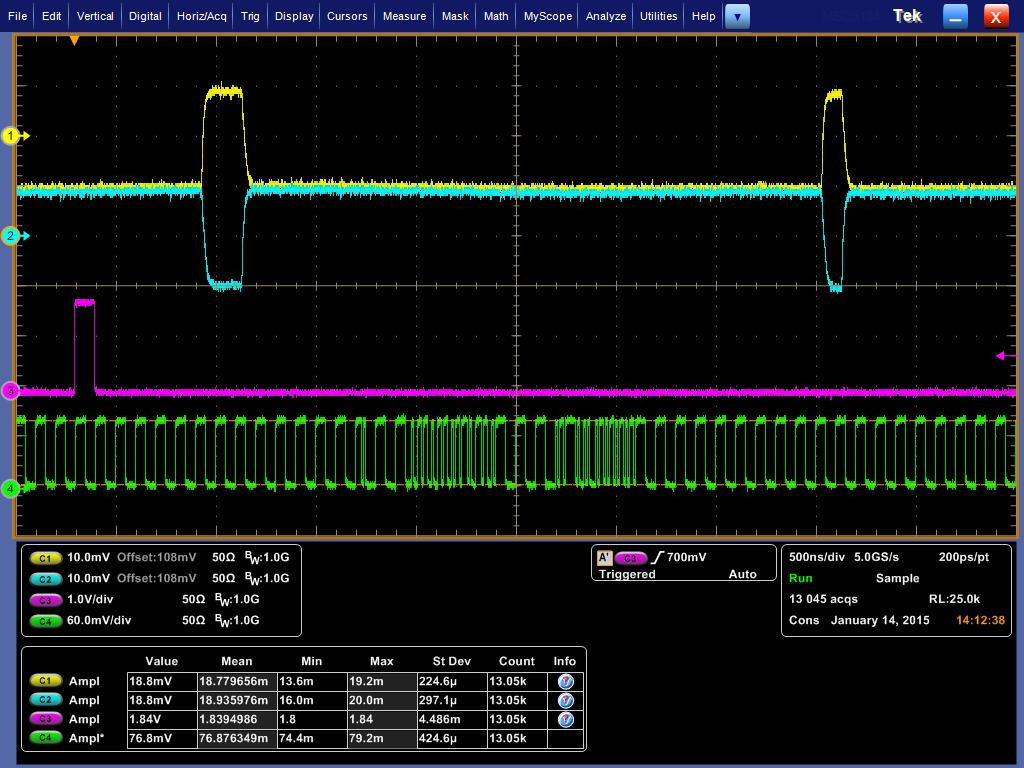
\includegraphics[width=0.7\textwidth]{figures/3_ctr.jpg}
 \caption{Oszilloskopbild beim CTR-Test.}
 \label{fig:ctrtest}
\end{figure}

Analog zum Clock-Test (Abschnitt~\ref{sec:clocktest}) ermitteln Sie die Signalamplituden im Oszilloskopkanal 1 und 2.
Vergessen Sie nicht den Oszilloskopspeicher f{\"u}r jede Messung erneut zur{\"u}ck zu setzen.
Die ermittelten \protokoll{Amplitudenwerte f{\"u}r Oszilloskopkanal 1 und 2} werden im Testprotokoll festgehalten.
Dieses Vorgehen wird f{\"u}r alle vier CTR-Signale wiederholt.


\subsection{SDA-Test}
Fahren Sie nun mit dem Test der Ausgabe serieller Daten (SDA) fort.
W{\"a}hlen Sie dazu an der ersten Signalweiche \frqq D2\flqq\ als Synchronisationssignal f{\"u}r das Oszilloskop und f{\"u}hren Sie folgendes Programm aus:
\begin{lstlisting}[style=console2]
 ./SDA[0,1,2,3]
\end{lstlisting}

Entsprechend der Wahl des SDA-Kanals, w{\"a}hlen Sie:
% \begin{lstlisting}[style=console1]
%  > select [{0,1,2,3},{4,5,6,7},{8,9,10,11},{12,13,14,15}]
% \end{lstlisting}
\begin{lstlisting}[style=console1]
 > select [0,4,8,12]
\end{lstlisting}

Stellen Sie das Oszilloskop mit der Taste Single auf den Einzelbild-Modus und f{\"u}hren Sie den folgenden Befehl aus:
\begin{lstlisting}[style=console1]
 > dac 25 70
\end{lstlisting}
Vergleichen Sie das Oszilloskopbild mit dem erwarteten Signalverlauf in Abbildung~\ref{fig:sdatest}:
\begin{figure}
\centering
  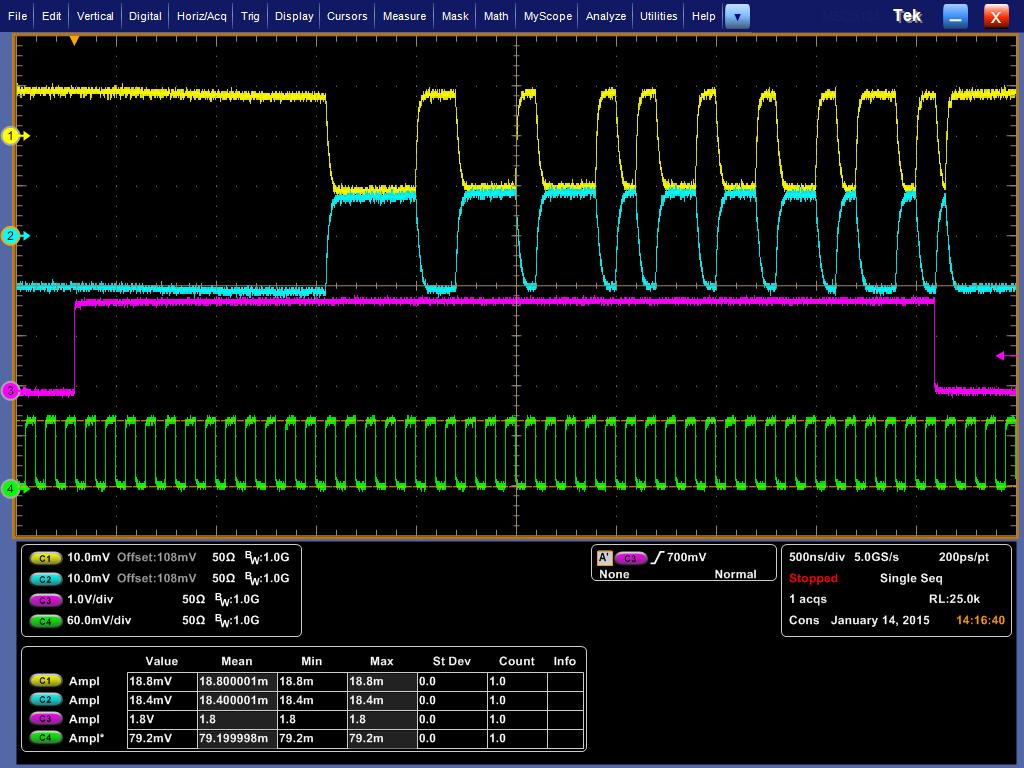
\includegraphics[width=0.7\textwidth]{figures/4_sda.jpg}
 \caption{Oszilloskopbild beim SDA-Test.}
 \label{fig:sdatest}
\end{figure}

Notieren Sie die \protokoll{Amplituden im Oszilloskopkanal 1 und 2} im Testprotokoll und wiederholen Sie die Prozedur f{\"u}r alle vier SDA-Kan{\"a}le.

\subsection{HV-Test}
Als letzten Test f{\"u}hren Sie den Hochspannungstest aus. Setzen Sie dazu zuerst die Relaiskarte zur{\"u}ck:
\begin{lstlisting}[style=console2]
 ./InitializeDigitalIO
\end{lstlisting}
Bitte beachten Sie, dass beim Hochspannungstest der \warnung{Messkopf unter keinen Umst{\"a}nden von dem HDI abgehoben werden darf}, da durch eine {\"U}berschlagsentladung das HDI und der Messkopf nachhaltig besch{\"a}digt werden k{\"o}nnen.
Generell ist w{\"a}hrend des gesamten Hochspannungstests jede Ber{\"u}hrung des HDI-Testers zu vermeiden.
Das Hochspannungsnetzteil sollte von Ihnen bereits auf eine Ausgangsspannung von 600V vorkonfiguriert sein.
Aktivieren Sie nun den Ausgangskanal mit der OPER-Taste am Hochspannungsnetzteil.
W{\"a}hlen Sie anschlie{\ss}end:
\begin{lstlisting}[style=console1]
 > hvon
\end{lstlisting}
Mit dem blauen Hochspannungsschalter schlie{\ss}en Sie letztlich den Stromkreis und Sie sollten nun im Display des Hochspannungsnetzteil einen Strom von einigen Microampere ablesen k{\"o}nnen.
Protokollieren Sie den \protokoll{gemessenen Strom} im Testprotokoll.
Das Ausschalten der Hochspannung erfolgt in umgekehrter Reihenfolge wie beim Einschalten:
Deaktivieren Sie den blauen Hochspannungsschalter und w{\"a}hlen Sie:
\begin{lstlisting}[style=console1]
 > hvoff
\end{lstlisting}
Deaktivieren Sie dann wieder die Ausgangsspannung am Hochspannungsnetzteil mit der OPER-Taste.
Da der Hochspannungstest der letzte elektronische Test des HDIs ist, schalten Sie nun auch die digitale Testbox aus und verlassen sie das Steuerprogramm mit:
\begin{lstlisting}[style=console1]
 > poff
 > exit
\end{lstlisting}

\section{Abschlie{\ss}ende Sichtkontrolle}
Bringen Sie den Messkopf am HDI-Tester vorsichtig in die Halteposition und sichern Sie diesen wieder mit der Arretierung.
Deaktivieren Sie die Vakuumpumpe und entnehmen Sie anschlie{\ss}end die Tr{\"a}gerplatte mit dem HDI aus dem HDI-Tester.
Das Flachkabel wird wieder vom HDI entfernt.
Pr{\"u}fen Sie zum Abschluss des HDI-Tests nochmals die \protokoll{wire-bonding Verbindungen} zum TBM-Chip mit einer Lupe oder dem Mikroskop und vermerken Sie das Ergebnis erneut im Testprotokoll.

\section{Au{\ss}erbetriebnahme}
Schalten Sie die Hochspannungsquelle und das Oszilloskop aus und warten Sie bis beide Ger{\"a}te vollst{\"a}ndig herunter gefahren sind, bevor Sie den Kippschalter an der Steckdosenleiste bet{\"a}tigen.

\appendix
\section*{Abk\"{u}rzungen}
\begin{acronym}[XXXXX]
 \acro{HDI}{high density interconnect}
 \acro{TBM}{token bit manager}
 \acro{CTR}{Calibration, Trigger, Reset}
 \acro{SDA}{Serial Data}
\end{acronym}
\end{document}          
